\chapter{Einleitung und Aufgabe}

Implementierung eines Webservice in PHP mit dem Slim Framework.

Zusatzaufgabe WS-Security gelöst durch Authentifizierung mittels OAuth2 und Verschlüsselung mittels HTTPS.

\chapter{Funktionen Webservice}

\begin{tabularx}{\columnwidth}{|X|p{1.5cm}|X|p{1.5cm}|}
	\hline
	Name & Method & URL & Access \\
	\hline
	\hline
	Alle verfügbare Fahrradstationen & GET & /stations & public \\
	\hline
	Spezielle Station & GET & /stations/stationID & public \\
	\hline
	Alle verfügbaren Fahrräder & GET & /bikes & public \\
	\hline
	Spezielles Fahrrad & GET & /bikes/bikesID & public \\
	\hline
	Alle Fahrradmodelle & GET & /models & public \\
	\hline
	Spezielles Fahrradmodell & GET & /models/modelID & public \\
	\hline
	Alle Buchungen & GET & /bookings & protected \\
	\hline
	Buchung erstellen & POST & /bookings & protected \\
	\hline
	Einzelne Buchung & GET & /bookings/bookingID & protected \\
	\hline
	Einzelne Buchung stornieren & DELETE & /bookings/bookingID & protected \\
	\hline
	Einzelne Buchung bearbeiten & PUT & /bookings/bookingID & protected \\
	\hline
	Accountinformationen & GET & /account & protected \\
	\hline
\end{tabularx}

\chapter{Webclient}

\begin{figure}
        \centering
	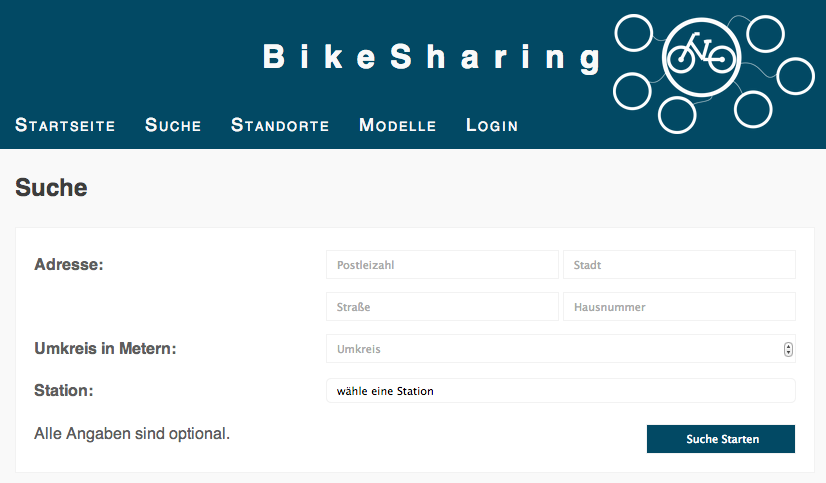
\includegraphics[height=80mm]{pics/bikesharing_search.png}
\end{figure}

\chapter{Zusatzaufgabe WS-Security}

\section{OAuth2}

Das Architekturkonzept von OAuth2 wird durch folgendes Schema verdeutlicht.

\begin{figure}
        \centering
	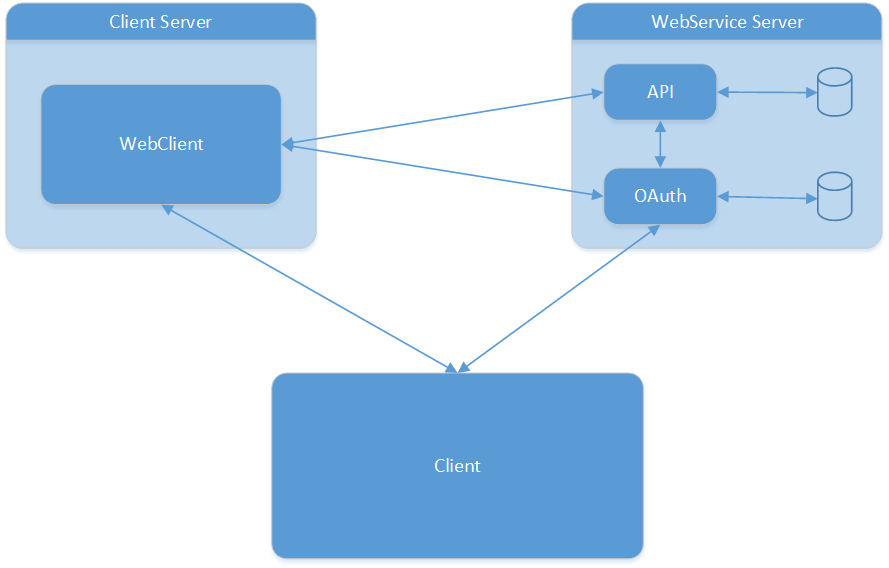
\includegraphics[height=80mm]{pics/Architektur.png}
\end{figure}

\section{Implementierung}

\chapter{Fazit}

Die Implementierung des Webclient ist nach Vorlage einer durchdachten API gut machbar.

Das Slim-Framework war eine gute Wahl, da die Verwendung sehr einfach und fehlerfrei verlief.
Die OAuth-Middleware hat leider nicht funktioniert.

Implementierung eines OAuth-Servers ist relativ kompliziert.


\chapter{Quellen}

